\documentclass[
	letterpaper, % Paper size, specify a4paper (A4) or letterpaper (US letter)
	10pt, % Default font size, specify 10pt, 11pt or 12pt
]{CSUniSchoolLabReport}

%----------------------------------------------------------------------------------------
%	REPORT INFORMATION
%----------------------------------------------------------------------------------------

\title{Controlling a Counter with Push Buttons by Hardware \\ Embedded Design: Enabling Robotics \\ EECE2160} % Report title

\author{Michael \textsc{Brodskiy}\\ \small \href{mailto:Brodskiy.M@Northeastern.edu}{Brodskiy.M@Northeastern.edu}}

\date{March 2, 2023} % Date of the report

%----------------------------------------------------------------------------------------


\begin{document}

\maketitle % Insert the title, author and date using the information specified above

\begin{center}
	\begin{tabular}{l r}
		Date Performed: & February 23, 2023 \\ % Date the experiment was performed
        Partner: & Dylan \textsc{Powers} \\ % Partner names
		Instructor: & Professor \textsc{Shazli} % Instructor/supervisor
	\end{tabular}
\end{center}

\newpage

\begin{abstract}

  The purpose of this laboratory experiment was to understand two central topics: clocks and debounce; through the use of clocks, timers (and, eventually, sequential circuits) can be constructed with ease. By employing debounce to push-buttons, the button will respond more accurately than without it.

\end{abstract}

\begin{flushleft}

  \textsc{Keywords:} \underline{clock}, \underline{debounce}, \underline{push-button}

\end{flushleft}

\newpage

\section{Equipment}

\hspace{.5 in} Available equipment included:\\

\begin{itemize}

  \item DE1-SoC board

  \item DE1-SoC Power Cable

  \item USB-A to USB-B Cable

  \item Computer

  \item Quartus Prime Schematic Software

\end{itemize}

\section{Introduction}

\hspace{.5 in} The goal of the lab was to showcase how to read the state of push buttons with hardware, and how to deal with debouncing effects introduced into the system with push buttons. The lab began with a simple design of a cascaded counter controlling an LED with the push button and then extended that cascaded counter design. The capabilities that were added included the ability to reset the counter, enable or disable the counters periodic increments, change the counting speed and change the counting direction. More specifically, the overall ability and switch assignment of the DE1-SoC board for this lab is shown below: \\

\begin{center}
\begin{tabular}[h!]{l r}
    KEY0: & Enable or disable counting \\
	KEY1: & Load counter value from switches\\
	KEY2: & Decrease counting speed \\
	KEY3: & Increase in counting speed\\
	SW[7..0]: &	Define the start value of the counter \\
	SW[8]: & Change the counting direction \\
\end{tabular}
\end{center}

\section{Pre-Lab}


\hspace{.5 in} The purpose of the Prelab was to provide a greater understanding of how push buttons work so they can be used in the lab assignment. A push button is a mechanical switch that when pressed closes contacts to establish continuity, In an ideal world, the continuity would be established immediately; however, due to elasticity present in the switch mechanism or contact materials, the push button contacts can ``bounce.'' This phenomenon is called contact ``bounce'' and happens in many switches, but oftentimes does not produce noticeable effects. If thinking about this strictly in terms of signals, a switch closing a contact can be thought of as a step function. When the switch is closed, the signal jumps to the desired value. Then, if contant bounce is present, instead of the signal jumping to the set value and staying there, the signal may oscillate from the reference to the set value and back a few times before settling on the set value. Essentially, the signal is being turned off and on until a permanent contact is established. \\\\
In cases when the bouncing is noticeable and undesired, actions must be taken for debouncing the switch. This can be done in many different ways, but for this lab, the debouncing will be done through settling the signal before the button is considered to have been effectively pressed. In order to do this, a cascade counter will be designed. Conceptually, the cascade counter will receive the bouncing signal, store the signal for a time that allows it to settle and then pass it along. 

\section{Discussion \& Analysis} 

\subsection{Assignment 1}

The goal of Assignment 1 was to design a cascaded counter in order to guarantee that a signal coming from the bush button has settled with a value of 1 for a long enough time before the push button is considered to be effectively pressed. In order to do this, two \textsc{LPM\_COUNTER} blocks were used with a \textsc{LPM\_COMPARE} block. The circuit that was created in the Quartus Prime Schematic Software is shown in Figure \ref{fig:1}.

\begin{figure}[H]
  \centering
  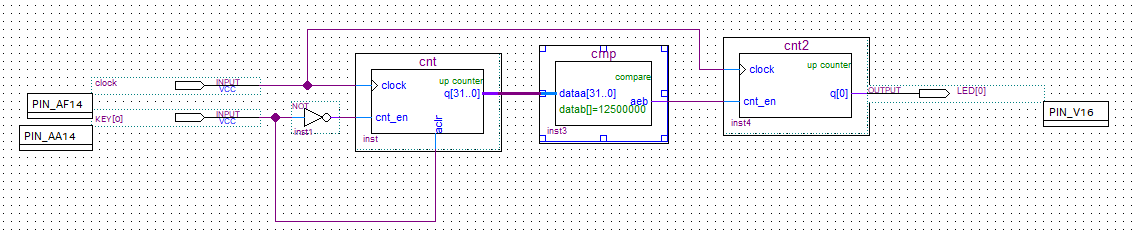
\includegraphics[width=.9\textwidth]{Figures/debounce_t.png}
  \caption{Turn LED ON/OFF with Push Button Design}
  \label{fig:1}
\end{figure}

\subsection{Assignment 2}

\hspace{.5 in} The goal of Assignment 2 was to design a free-running 8-bit cascaded counter. For this counter, the outputs were connected to the first eight LEDs on the DE1-SoC board and the 7-Segment displays on the board. Then whenever the counter transitioned to a new state, both the LEDs and the 7-Segment displays reflected the new count value. Given that the DE1-SoC’s FPGA has a default clock frequency of 50,000,000 Hz, a cascaded counter was used to ensure that the values were not changing instantaneously. The design for Assignment 2 is displayed in Figure \ref{fig:2}.

\begin{figure}[H]
  \centering
  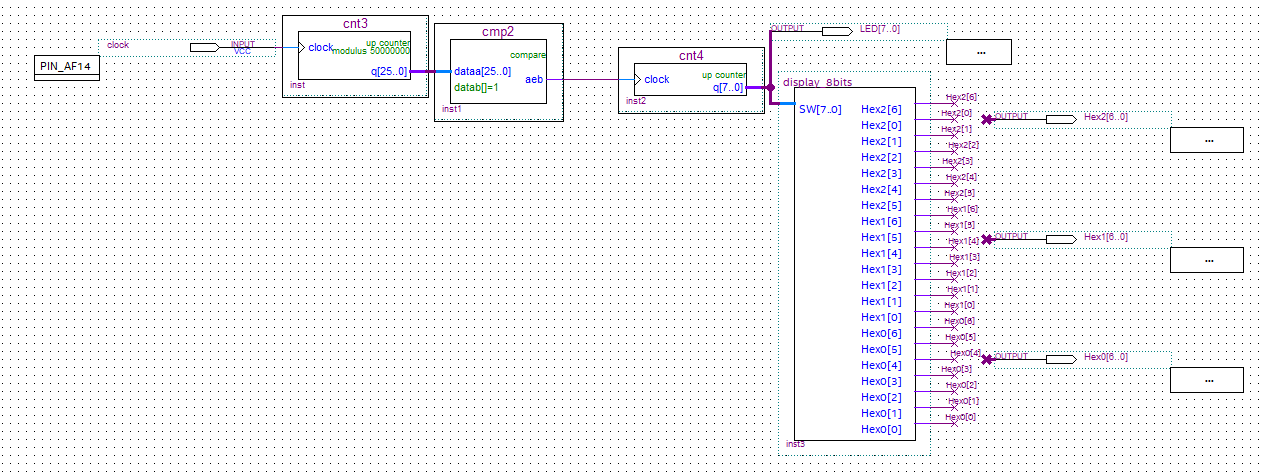
\includegraphics[width=.72\textwidth]{Figures/Assign2.png}
  \caption{Free-Running 8-bit Cascaded Counter}
  \label{fig:2}
\end{figure}

\subsection{Assignment 3}

\hspace{.5 in} The goal of Assignment 3 was to take the previously designed cascaded counter in Assignment 2, and implement a KEY0 operation to be able start or stop the counter using the appropriate debounce system. In order to achieve this functionality, the timing counter (50MHz counter) block was double clicked to bring up settings of the counter.  The settings were then changed to add the Count Enable port which a KEY0 input into a NOT gate was connected to. Therefore, when the KEY0 button was pressed it sent a 1 to the enable input of the rightmost counter, which turned on the counter. Then when the KEY0 pushbutton was released, the counter would be diables and stop counting. An image of the design can be seen in Figure \ref{fig:3}.

\begin{figure}[H]
  \centering
  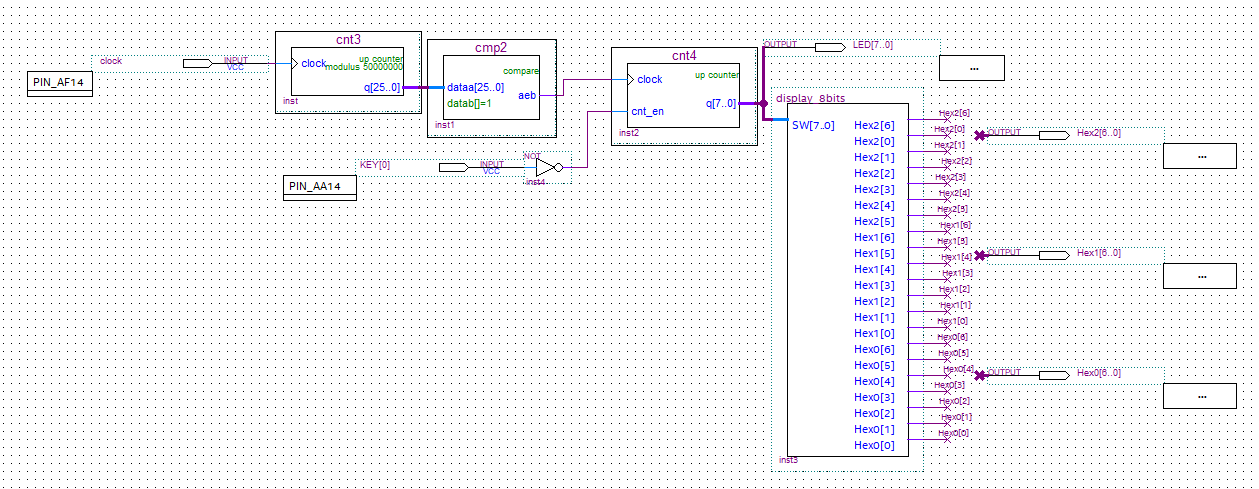
\includegraphics[width=.72\textwidth]{Figures/Assign3.png}
  \caption{Start/Stop 8-bit Cascaded Counter}
  \label{fig:3}
\end{figure}

\subsection{Assignment 4}

\hspace{.5 in} The goal of Assignment 4 was to expand the design from Assignment 3 and allow for the ability to toggle the direction of the counting based on the position of SW[8]. If the switch 8 was OFF then the counter counted towards 255 and if the switch was ON, the counter would count towards 0. To achieve this objective, the 8-bit counter was double clicked to view the settings, which were changed to to have an additional up/down input port on the \textsc{LPM\_COUNTER}. Once the port was added, the switch 8 input was added to it with a NOT gate. The NOT gate was added due to the fact that the counter needed to count upwards when switch 8 was 0 and count downwards when switch 8 was 1. Without the NOT gate, the functionality of the counter would have been opposite of what was desired. Shown below is the circuit design that was created in the Quartus Prime Schematic Software.

\begin{figure}[H]
  \centering
  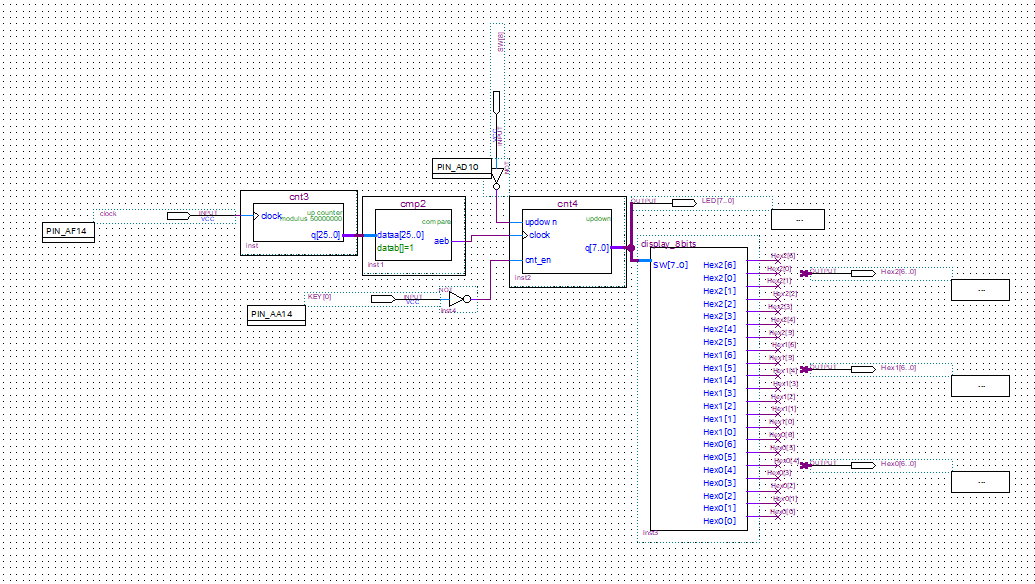
\includegraphics[width=.72\textwidth]{Figures/Assign4.png}
  \caption{Extended Design to Toggle Counting Direction with SW[8]}
  \label{fig:4}
\end{figure}

\subsection{Assignment 5}

\hspace{.5 in} The final integration in this lab was the inclusion of a ``load value'' feature. Switches 7 through 0 (SW[7..0]) were used to input an eight-bit binary number. This number would then, upon the press of push-button 1 (KEY[1]) be loaded into the timer, and, upon pressing the other push-button (KEY[0]), the timer would resume counting from the loaded number, in the direction specified by SW[8].

\begin{figure}[H]
  \centering
  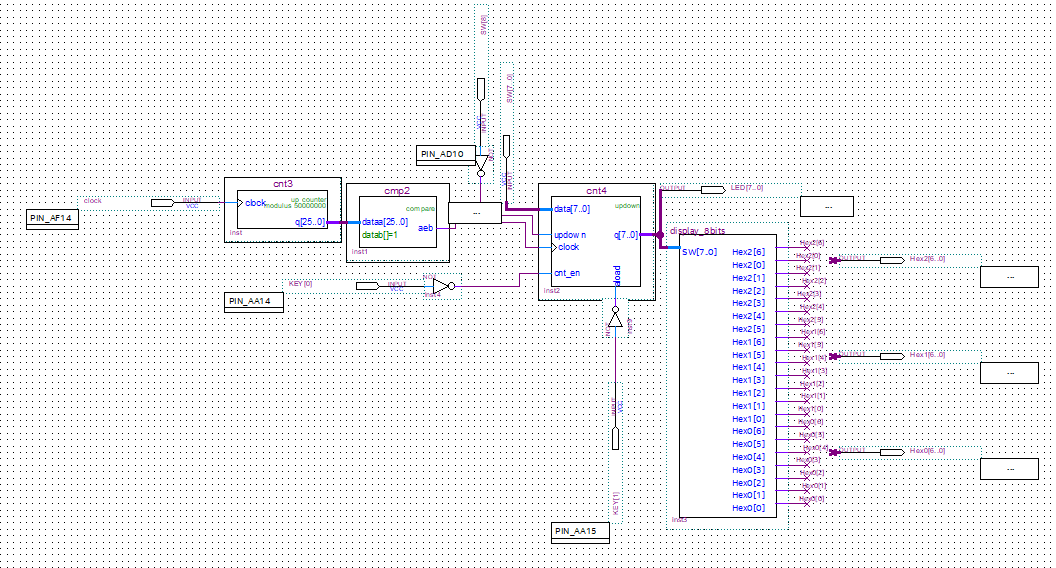
\includegraphics[width=.72\textwidth]{Figures/Assign5.png}
  \caption{Further Extended Design to addd Load Value Functionality Using SW[7..0]}
  \label{fig:4}
\end{figure}


\section{Conclusion}

\hspace{.5 in} Overall, this lab resulted in the construction of push-button-manipulated, switch-configured 8-bit counter, which employed the on-board 50$[\si{\mega\hertz}]$ clock. In this manner, we were able to employ the concept of clocks to control the timer, in tandem with the concept of debounce to add precision to push-button response.

\end{document}
